\documentclass[11pt]{article}

\usepackage[margin=1in]{geometry}
\usepackage{amsmath,amssymb,amsthm}
\usepackage{graphicx}
\usepackage{booktabs}
\usepackage{xcolor}
\usepackage[numbers,sort&compress]{natbib}
\usepackage[colorlinks=true,linkcolor=black,citecolor=blue,urlcolor=blue]{hyperref}

\graphicspath{{figures/}}
\setlength{\emergencystretch}{2em}
\newcommand{\err}{\mathrm{err}}
\newcommand{\qhat}{\hat{q}}

\title{\bfseries Conformal Prediction for Financial Returns:\\
Where Coverage Survives and Where It Breaks}

\author{Eugen Soloviov\thanks{Independent Researcher. ORCID:
\href{https://orcid.org/0009-0006-3148-111X}{0009-0006-3148-111X}.
Correspondence: \href{mailto:suenot@gmail.com}{suenot@gmail.com}.
Code to reproduce every number and figure:
\url{https://github.com/suenot/conformal-coverage}.}}

\date{}

\begin{document}
\maketitle

\begin{abstract}
Conformal prediction promises finite-sample marginal coverage under
exchangeability---a property financial returns conspicuously lack. We give the
claim that ``conformal transfers to returns'' a controlled accounting on
simulated processes whose true conditional quantiles are known exactly: iid,
AR(1), GARCH(1,1), and abrupt regime breaks ($180$ experiments, $14$ interval
methods, nominal $90\%$, online protocol). The verdict splits. \emph{Marginal}
coverage survives stationary dependence almost exactly: split conformal covers
$0.901/0.901/0.895$ on iid/AR(1)/GARCH, only the break DGP dents it
($0.877$), and Adaptive Conformal Inference (ACI) sits at $0.900$ everywhere.
\emph{Conditional} and \emph{post-break} coverage are where it breaks: under
GARCH the absolute-score interval covers $0.952/0.915/0.820$ across
true-volatility terciles---under-covering by $8$ points exactly when a
position sizer most needs honesty; normalizing the score by an EWMA volatility
closes the spread from $0.134$ to $0.040$, while conformalized quantile
regression is only a partial fix. After a break, first-$60$-step coverage
drops to $0.562$; ACI repairs the hole monotonically in its learning rate
($0.700$--$0.875$) at a width cost of $1.12$--$1.14\times$ oracle. At matched
coverage, honesty costs width: the parametric Gaussian--EWMA baseline is
narrowest ($0.99$--$1.03\times$) but pays with quiet under-coverage
($0.878$--$0.888$). A side finding corrects folklore: at the $90\%$ level,
fat tails make a correctly-scaled Gaussian interval \emph{over}-cover. The
recipe: normalize conformal scores by a volatility proxy, add ACI when breaks
are a concern, and treat parametric narrowness as a coverage liability until
proven otherwise.
\end{abstract}

\section{Introduction}

A trading system that sizes positions from a $90\%$ prediction interval needs
that interval to cover $90\%$ of outcomes---not on average over a backtest, but
\emph{tonight}, in the volatility regime it is actually in. Conformal
prediction \citep{vovk2005algorithmic,shafer2008tutorial} is increasingly
recommended for this job because it wraps any forecaster in a calibration step
with a finite-sample marginal coverage guarantee and no distributional
assumptions. The guarantee, however, is proved under exchangeability, and
financial returns violate it in every interesting way: volatility clusters,
means drift, regimes break. A growing body of practitioner writing asserts
that the method transfers anyway.\footnote{The specific practitioner advice
under test here---including the claim that split conformal transfers to
returns essentially unchanged, the EWMA-normalized score, and an ACI variant
for regime shifts---originates in the author's own earlier practitioner draft
(a market-making blog post on conformal prediction for position sizing). This
paper is therefore a controlled \emph{self-audit} of advice the author has
himself circulated, not an attack on a third party. The audit caught a
concrete bug: the draft's ACI pseudocode updates the conformal quantile with a
sign such that a \emph{missed} interval \emph{narrows} the next one---the
opposite of the Gibbs--Cand\`es recursion. The corrected update
(Eq.~\ref{eq:aci}) is pinned by a unit test in the released code.}

Whether it does is an empirical question with a measurable answer, because the
failure modes are specific. Exchangeability violations can hurt in three
distinct currencies: marginal coverage (the average), conditional coverage
(the average within a volatility regime), and transient coverage (the weeks
after a structural break). Theory says little about how large each effect is
in practice, and published experiments rarely separate them. We separate them
by construction: we simulate from four return DGPs whose true conditional
quantiles are \emph{exactly} computable---iid, AR(1) mean, GARCH(1,1), and an
abrupt regime break---and run an online protocol (rolling refits, sliding
calibration window, one-step-ahead intervals) over $14$ methods: split
conformal with absolute and volatility-normalized scores, conformalized
quantile regression (CQR), Adaptive Conformal Inference (ACI) at four learning
rates on both scores, an unconformalized quantile regression, a parametric
Gaussian--EWMA interval, and the oracle. Every coverage number below is
measured against known truth, and every DGP parameter is sampled from
documented ranges and recorded.

Our findings are deliberately split rather than a blanket verdict. Marginal
coverage is far more robust to stationary dependence than the exchangeability
caveat suggests---and far less robust to breaks. Conditional coverage is the
real casualty, and it is repairable at almost no cost. The parametric
benchmark every finance reader will ask about is genuinely narrower, but the
narrowness is financed by under-coverage.

\paragraph{Contributions.}
\begin{enumerate}\itemsep2pt
\item A reproducible simulation framework of four financial DGPs with exactly
computable true conditional intervals, an online evaluation protocol, and a
fully sampled-and-recorded design ($180$ experiments $\times$ $14$ methods
$=2{,}520$ method-rows), so marginal, regime-conditional, and post-break
coverage are measured against ground truth (Sections~\ref{sec:framework}--\ref{sec:setup}).
\item A marginal-coverage accounting across dependence types: the
exchangeability gap of split conformal is $-0.005$ $[-0.007,-0.003]$ under
GARCH and $-0.023$ $[-0.024,-0.021]$ under abrupt breaks; ACI holds $0.900$
on every DGP, empirically confirming its distribution-free guarantee
(Section~\ref{sec:marginal}).
\item The headline conditional-coverage accounting on GARCH: the absolute
score covers $0.952/0.915/0.820$ by true-volatility tercile; an EWMA-normalized
score closes the spread from $0.134$ to $0.040$ (paired $+0.094$), lifting
high-volatility coverage by $+0.085$; CQR recovers less than half as much
(Section~\ref{sec:conditional}).
\item An anatomy of the post-break coverage hole and its repairs: depth,
duration ($\approx$ the calibration window), the monotone ACI
$\gamma$-vs-width trade-off, and the finding that volatility normalization
alone repairs most of the hole for volatility breaks
(Section~\ref{sec:breaks}).
\item A width-at-matched-coverage comparison against a parametric
Gaussian--EWMA baseline, plus a correction to the ``Gaussian intervals
under-cover fat tails'' folklore at central coverage levels
(Sections~\ref{sec:width}--\ref{sec:tails}).
\end{enumerate}

\section{Related work}
\label{sec:related}

\textbf{Conformal prediction under exchangeability.} Conformal prediction
originates in the on-line compression framework of \citet{vovk2005algorithmic},
whose second edition consolidates two further decades of development
\citep{vovk2022algorithmic}. The method wraps any point predictor in a
calibration step that converts nonconformity scores into prediction sets with
finite-sample marginal coverage, requiring only exchangeability of the
data---no model correctness, no distributional assumptions.
\citet{shafer2008tutorial} give the canonical tutorial treatment, and
\citet{angelopoulos2023conformal} provide a modern introduction oriented toward
practitioners. The split (inductive) variant we benchmark was analyzed in
depth by \citet{lei2018distribution}, who establish distribution-free marginal
validity for regression and, crucially for our purposes, also prove that
\emph{conditional} validity is unattainable in finite samples without further
assumptions. This marginal-versus-conditional distinction is the fault line
our experiments are designed to expose: financial returns are precisely the
setting where marginal coverage can be honest on average while being
systematically wrong in every volatility regime.

\textbf{Adaptivity to heteroskedasticity.} Within the exchangeable setting, a
second line of work makes interval \emph{width} responsive to the input.
\citet{romano2019conformalized} conformalize quantile regression (CQR),
calibrating intervals built from estimated conditional quantiles and
inheriting both the finite-sample guarantee and the local adaptivity of the
base learner; locally weighted (normalized) nonconformity scores in
\citet{lei2018distribution} pursue the same goal by rescaling residuals with a
dispersion estimate---the direct ancestor of the volatility-normalized
conformal method we evaluate. \citet{chernozhukov2021distributional} push
further with distributional conformal prediction, ranking
probability-integral-transform values rather than raw residuals; notably,
their empirical motivation is a daily stock-return exercise in which the
coverage of a mean-residual conformal interval collapses to roughly $50\%$ in
high-volatility periods. That observation is, to our knowledge, the closest
published precedent for our regime-stratified accounting, but it appears as a
motivating illustration rather than a systematic study.

\textbf{Conformal prediction beyond exchangeability.} Serial dependence breaks
exchangeability, and a substantial literature now relaxes it.
\citet{chernozhukov2018exact} introduce block-permutation conformal inference
and prove approximate validity for strongly mixing time series.
\citet{xu2021conformal} propose EnbPI, an ensemble-bootstrap construction with
asymptotic marginal coverage under mixing errors and no data splitting.
\citet{barber2023conformal} drop exchangeability entirely, deriving a coverage
gap bound for weighted conformal prediction governed by the total-variation
distance between the test point and the (downweighted) calibration points. In
the online setting, \citet{gibbs2021adaptive} introduce Adaptive Conformal
Inference (ACI), which tunes the working miscoverage level by online gradient
descent and guarantees the correct long-run coverage \emph{frequency} for
arbitrary, even adversarial, distribution shift; \citet{gibbs2024conformal}
strengthen this to coverage guarantees that hold simultaneously over arbitrary
subintervals and covariate subsets. \citet{zaffran2022adaptive} analyze ACI's
learning-rate sensitivity on dependent series and propose the
expert-aggregation variant AgACI. A common thread deserves emphasis: each
relaxation purchases validity in a \emph{weaker currency}---asymptotic,
approximate, long-run-averaged, or TV-bounded---and the papers' experiments
(electricity prices, ozone, synthetic mixing processes) rarely interrogate
what those weaker guarantees deliver pathwise, conditionally on a volatility
regime, or in the window immediately following a structural break.

\textbf{Volatility models and interval evaluation in econometrics.} Finance
has its own mature answer to predictive intervals. The ARCH and GARCH models
of \citet{engle1982autoregressive} and \citet{bollerslev1986generalized} yield
conditional-variance forecasts whose implied intervals adapt to volatility
clustering by construction---the natural parametric baseline that any conformal
method applied to returns must beat or at least match. Equally relevant is the
econometric tradition of \emph{testing} interval forecasts:
\citet{kupiec1995techniques} tests unconditional coverage of VaR exceptions,
and \citet{christoffersen1998evaluating} adds the conditional-coverage and
independence tests that detect exactly the failure mode conformal marginal
guarantees permit---correct average coverage with clustered violations. We
import the spirit of that toolkit: our regime-stratified and post-break
accounting asks Christoffersen's question---is coverage right
\emph{conditionally}, not just on average?---but answers it against exact
ground truth rather than through asymptotic tests on real data.

\textbf{The gap.} The two literatures pass each other by.
Conformal-for-time-series theory papers
\citep{chernozhukov2018exact,xu2021conformal,barber2023conformal,gibbs2021adaptive,gibbs2024conformal,zaffran2022adaptive}
prove validity under specific relaxations of exchangeability and validate on
whatever applications are at hand, while a growing body of finance-facing
explainer and applied content simply asserts that conformal methods transfer
to returns. What is missing is a controlled accounting: simulations from
financial DGPs---AR, GARCH, and regime-shift processes---where the true
conditional quantiles are known exactly, so that marginal coverage,
volatility-regime-conditional coverage, and post-break coverage can each be
measured against ground truth rather than proxied. Such a design answers
questions the theory leaves open in practice: how badly split conformal
under-covers in high-volatility regimes and over-covers in calm ones; how much
of that gap volatility normalization and CQR actually recover; how many
observations ACI needs to re-cover after a break and at what cost in interval
width; and---the question finance practitioners actually face---whether any of
this outperforms a plain interval from a fitted volatility model
\citep{bollerslev1986generalized}, judged by the field's own coverage criteria
\citep{christoffersen1998evaluating,kupiec1995techniques}. This paper supplies
that accounting.

\section{Interval methods}
\label{sec:methods}

All methods target the central interval at nominal level $1-\alpha$ with
$\alpha=0.10$. Throughout, $\hat\mu(x)$ is a point forecast and
$\hat{q}_{\mathrm{lo}}(x),\hat{q}_{\mathrm{hi}}(x)$ are conditional-quantile
forecasts at levels $\alpha/2$ and $1-\alpha/2$, all produced by gradient
boosting on causal features of past returns (Section~\ref{sec:setup}).

\paragraph{Split conformal with the finite-sample correction.} Given $n$
calibration scores $s_1,\dots,s_n$, define the conformal quantile
\begin{equation}
\qhat_\alpha \;=\; s_{(\lceil (1-\alpha)(n+1)\rceil)},
\label{eq:cq}
\end{equation}
the $\lceil (1-\alpha)(n+1)\rceil$-th order statistic, with
$\qhat_\alpha=+\infty$ when the corrected rank exceeds $n$ (the honest
``infinite interval'' case). With the absolute-residual score
$s_i=|y_i-\hat\mu(x_i)|$ the interval is
$C_t=[\hat\mu(x_t)-\qhat_\alpha,\;\hat\mu(x_t)+\qhat_\alpha]$
(\texttt{split\_abs}). If the $n+1$ scores are exchangeable,
$1-\alpha \le \mathbb{P}(y_{n+1}\in C) \le 1-\alpha + 1/(n+1)$
\citep{lei2018distribution} (the upper bound assuming almost-surely distinct
scores, which holds for our continuous scores); with our calibration window $n=250$ the
theoretical coverage is $\lceil 0.9\cdot 251\rceil/251 \approx 0.9004$.

\paragraph{Volatility-normalized score.} The locally weighted variant
\citep{lei2018distribution} divides the residual by a dispersion estimate:
$s_i=|y_i-\hat\mu(x_i)|/\hat\sigma_i$, giving
$C_t=\hat\mu(x_t)\pm \qhat_\alpha\,\hat\sigma_t$ (\texttt{split\_norm}). We
use the practitioner's cheapest dispersion estimate, a RiskMetrics-style EWMA
$\hat\sigma_t^2=\lambda\hat\sigma_{t-1}^2+(1-\lambda)r_{t-1}^2$ computed from
past returns only.

\paragraph{Conformalized quantile regression.} CQR
\citep{romano2019conformalized} scores
$s_i=\max\{\hat{q}_{\mathrm{lo}}(x_i)-y_i,\;y_i-\hat{q}_{\mathrm{hi}}(x_i)\}$
and reports
$C_t=[\hat{q}_{\mathrm{lo}}(x_t)-\qhat_\alpha,\;\hat{q}_{\mathrm{hi}}(x_t)+\qhat_\alpha]$,
inheriting the width adaptivity of the quantile learner.

\paragraph{Adaptive conformal inference.} ACI \citep{gibbs2021adaptive} keeps
the conformal machinery but tunes the \emph{working level} $\alpha_t$ online:
\begin{equation}
\alpha_{t+1} \;=\; \alpha_t + \gamma\,(\alpha - \err_t),
\qquad
\err_t = \mathbf{1}\{y_t \notin C_t\},
\label{eq:aci}
\end{equation}
so a miss ($\err_t=1$) \emph{lowers} $\alpha_t$ and widens the next interval,
and a hit tightens it.\footnote{Note the direction; the practitioner draft
audited here got it backwards (see the footnote in the Introduction). When
$\alpha_t$ wanders to $\le 0$ the corrected rank in Eq.~\eqref{eq:cq} exceeds
$n$ and the interval is all of $\mathbb{R}$ (always covers); when
$\alpha_t\ge 1$ it is empty. Both conventions are required by the ACI
guarantee; in our released runs only the always-cover case ever occurs (the
empty-interval case never triggers), and the fraction of unbounded steps is
reported wherever it is non-negligible.} For \emph{any} data sequence,
$|\frac{1}{T}\sum_{t\le T}\err_t-\alpha|\le
(\max(\alpha_1,1-\alpha_1)+\gamma)/(\gamma T)$; at our test length $T=1500$
the bound is $0.121/0.061/0.031/0.013$ for
$\gamma=0.005/0.01/0.02/0.05$. We run ACI on top of both the absolute and the
normalized score at all four $\gamma$ values.

\paragraph{Baselines and oracle.} \texttt{raw\_qr} reports the
unconformalized quantile-regression band
$[\hat{q}_{\mathrm{lo}},\hat{q}_{\mathrm{hi}}]$---what a practitioner gets by
skipping calibration. \texttt{param\_gauss} is the parametric benchmark: a
Gaussian interval $\hat\mu(x_t)\pm z_{1-\alpha/2}\,\hat\sigma_t^{\mathrm{QML}}$
whose EWMA decay is refit on each training window by Gaussian
quasi-maximum-likelihood over the grid $\lambda\in\{0.80,0.81,\dots,0.99\}$%
---an IGARCH/RiskMetrics-style stand-in for the GARCH tradition
\citep{engle1982autoregressive,bollerslev1986generalized}. \texttt{oracle} is
the DGP's true conditional interval, the efficiency yardstick: all widths
below are reported as ratios to it.

\section{Simulation framework}
\label{sec:framework}

Every DGP emits returns of the form
\begin{equation}
r_t \;=\; \mu_t + \sigma_t\, z_t,
\label{eq:dgp}
\end{equation}
where $z_t$ are i.i.d.\ \emph{standardized} (zero-mean, unit-variance)
innovations---Gaussian, or Student-$t$ with $\nu\in\{4,6,10\}$ scaled by
$\sqrt{(\nu-2)/\nu}$---and $(\mu_t,\sigma_t)$ are the true conditional mean
and standard deviation given the past. The true conditional interval at level
$1-\alpha$ is therefore exactly
$[\mu_t+\sigma_t F_z^{-1}(\alpha/2),\;\mu_t+\sigma_t F_z^{-1}(1-\alpha/2)]$ at
every step, which is what makes coverage exactly measurable. Four processes
span the failure modes (Figure~\ref{fig:setup}):
\begin{itemize}\itemsep2pt
\item \textbf{iid}: constant $(\mu,\sigma)$---the exchangeable base case where
the split-conformal theorem applies verbatim.
\item \textbf{AR(1)}: predictable mean $\mu_t=\mu+\phi\,(r_{t-1}-\mu)$,
constant $\sigma$ (dependence without heteroskedasticity).
\item \textbf{GARCH(1,1)}: $\sigma_t^2=\omega+a\,(r_{t-1}-\mu)^2+b\,\sigma_{t-1}^2$
with $\omega=\sigma^2(1-a-b)$ \citep{bollerslev1986generalized}---volatility
clustering; stationary but not exchangeable. The true $\sigma_t$ comes from
the recursion itself.
\item \textbf{break}: iid base with an abrupt shift at step $t^\ast$:
$\sigma\to\kappa\sigma$ and/or $\mu\to\mu+\delta$.
\end{itemize}

\paragraph{Sampled design (nothing hidden).} Each experiment draws its DGP
from documented ranges, all recorded in the released per-experiment records:
base volatility $\sigma\sim\mathrm{LogUniform}[0.005,0.02]$ per step; drift
$\mu\sim\mathrm{Uniform}[-0.1\sigma,0.1\sigma]$; Student-$t$ innovations with
probability $0.5$ ($\nu$ uniform on $\{4,6,10\}$);
$\phi\sim\mathrm{Uniform}[0.1,0.5]$;
$a\sim\mathrm{Uniform}[0.05,0.20]$ and $b\sim\mathrm{Uniform}[0.70,0.92]$ with
$a+b$ capped at $0.97$; break type volatility/mean/both with probabilities
$0.4/0.2/0.4$, volatility multiplier $\kappa\in\{2,4\}$, mean shift
$\delta=\pm\mathrm{Uniform}[1,2]\cdot\sigma$, and break time uniform over the
$[30\%,60\%]$ stretch of the test segment so post-break behavior is always
observable. The full batch runs $36/36/48/60$ experiments on
iid/AR(1)/GARCH/break (more where the questions live), i.e.\ $180$
experiments; realized innovation splits are $20/16$, $13/23$, $31/17$, and
$32/28$ Gaussian/Student-$t$ respectively. With $14$ method-rows per
experiment the result set has $2{,}520$ rows. Everything is deterministic
given the released seed ($20260610$); the full batch takes about six minutes
on one core.

\begin{figure}[t]
\centering
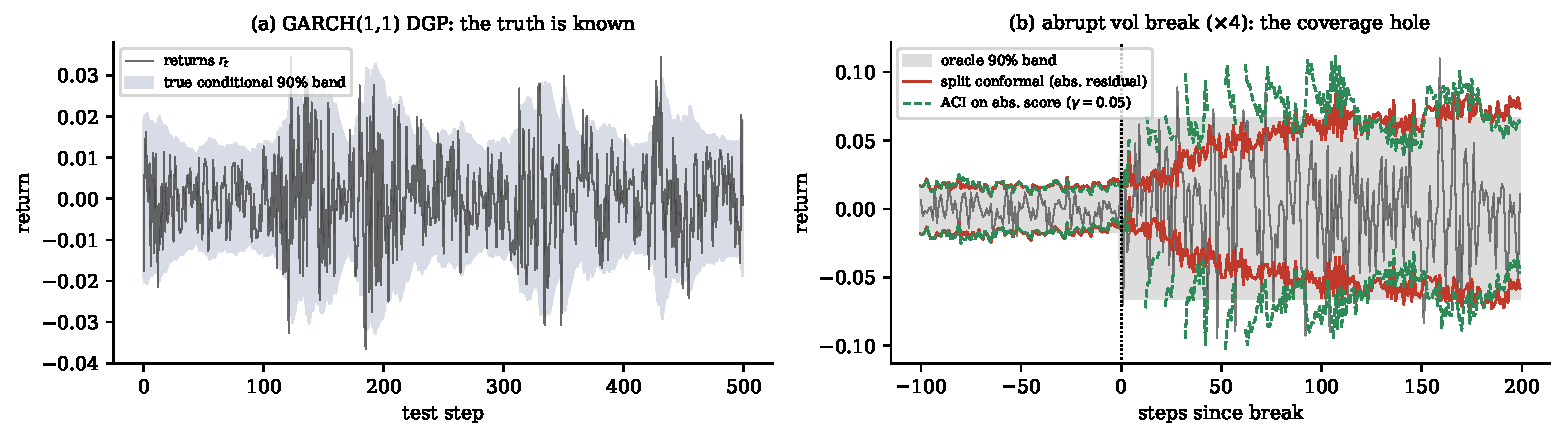
\includegraphics[width=\textwidth]{fig_setup.pdf}
\caption{The testbed. (a) A GARCH(1,1) path with its \emph{true} conditional
$90\%$ band---known exactly because we simulate, so coverage is measured, not
proxied. (b) An abrupt $\times 4$ volatility break: the oracle band widens
instantly; the split-conformal interval (absolute residual) stays at
pre-break width until its calibration window turns over---the coverage
hole---while ACI ($\gamma=0.05$) widens within steps by reacting to its own
misses. Both panels use illustrative parameters that feed no quantitative
result.}
\label{fig:setup}
\end{figure}

\section{Experimental setup}
\label{sec:setup}

\paragraph{Online protocol.} Each experiment walks forward through
$1{,}500$ test steps producing a one-step-ahead interval from every method at
every step. The learners are refit every $250$ steps on the $600$
observations immediately preceding the calibration window (so a model can be
up to ${\sim}500$ steps stale at the end of a refit block); the calibration
set is the most recent $250$ nonconformity
scores, re-scored under the model currently in force and slid forward every
step (newly observed outcomes enter immediately). ACI states update every
step from the realized cover/miss of their own interval, as in
\citet{gibbs2021adaptive}. The point and quantile learners are gradient
boosting machines ($100$ trees, depth $2$, learning rate $0.08$; quantile loss
for $\hat{q}_{\mathrm{lo}},\hat{q}_{\mathrm{hi}}$) over strictly causal
features: five lagged returns, $|r_{t-1}|$, a rolling mean, rolling standard
deviations over windows $5$ and $20$, and an EWMA volatility. The EWMA decay
used by the normalized score is itself sampled per experiment,
$\lambda\sim\mathrm{Uniform}[0.90,0.97]$, so results do not hinge on a tuned
constant. The true $(\mu_t,\sigma_t)$ are used only for scoring and the
oracle; no learner ever sees them.

\paragraph{Metrics.} For each experiment and method we record marginal
coverage; mean width as a per-step ratio to the oracle width; coverage and
width stratified by \emph{true}-volatility tercile (terciles of $\sigma_t$
within the test path---defined whenever $\sigma_t$ varies); the tercile
coverage spread (max minus min); for break experiments, coverage in the
event-time windows $0$--$60$, $60$--$150$, $150$--$300$, $300$--$600$ after
the break, the \emph{hole depth} (minimum of the rolling-$60$-step coverage
after the break), and the \emph{recovery time} (first step at which
rolling-$60$ coverage returns above $1-\alpha-0.03=0.87$); and the fraction
of unbounded (infinite) intervals, which only ACI can produce. Aggregates are
means over experiments with normal-approximation $95\%$ confidence intervals;
paired method comparisons difference the per-experiment values. We never
report an aggregate whose stratified breakdown reverses it.

\section{Results}
\label{sec:results}

\subsection{Marginal coverage survives stationary dependence almost exactly}
\label{sec:marginal}

Table~\ref{tab:marginal} and Figure~\ref{fig:marginal} give the marginal
accounting. On iid data split conformal delivers its theorem: coverage
$0.901$ against the theoretical $0.9004$. The interesting cells are the
non-exchangeable ones. Under AR(1) dependence the gap is statistically
invisible ($+0.001$, with a CI of $[-0.000,+0.003]$ that includes zero). Under GARCH---where consecutive
scores are strongly dependent through the volatility state---the gap is real
but tiny: coverage $0.895$, a gap of $-0.005$ $[-0.007,-0.003]$. For marginal
coverage under \emph{stationary} dependence, the exchangeability caveat is, at
this sample size, a rounding error.

Breaks are different in kind: split-absolute drops to $0.877$ (gap $-0.023$
$[-0.024,-0.021]$)---modest on average only because the test window is long;
Section~\ref{sec:breaks} shows the damage is concentrated. Three further
observations. First, ACI is the marginal-coverage instrument its theorem
promises: across every DGP, score, and $\gamma$, its coverage lies in
$[0.900,0.901]$---deviations from nominal at least an order of magnitude
inside the worst-case bounds of Section~\ref{sec:methods}. Second, the
\emph{normalized} split conformal is marginally clean everywhere
\emph{including} breaks ($0.902$): the EWMA proxy in the score tracks the
volatility jump within steps, so the calibration distribution barely moves.
Third, conformalization is doing real work: the raw quantile-regression band
under-covers everywhere ($0.884/0.882/0.875$ on iid/AR(1)/GARCH) and collapses
to $0.753$ on breaks, and the parametric Gaussian--EWMA baseline under-covers
on three of four DGPs ($0.891/0.881/0.883$ on iid/GARCH/break).

\begin{table}[t]
\centering
\caption{Marginal coverage by method and DGP (nominal $0.90$; mean over
experiments). All eight ACI variants ($\gamma\in\{0.005,0.01,0.02,0.05\}$,
both scores) lie in $[0.900,0.901]$ on every DGP; the two $\gamma=0.01$ rows
are shown. Oracle coverage deviates from $0.900$ only by Monte-Carlo noise.}
\label{tab:marginal}
\small
\begin{tabular}{lcccc}
\toprule
Method & iid & AR(1) & GARCH & break \\
\midrule
Oracle (true quantiles)            & 0.899 & 0.901 & 0.898 & 0.902 \\
Split conformal (absolute)         & 0.901 & 0.901 & 0.895 & 0.877 \\
Split conformal (normalized)       & 0.900 & 0.902 & 0.901 & 0.902 \\
CQR                                & 0.901 & 0.901 & 0.896 & 0.878 \\
ACI, abs.\ score ($\gamma{=}0.01$) & 0.900 & 0.900 & 0.901 & 0.900 \\
ACI, norm.\ score ($\gamma{=}0.01$)& 0.900 & 0.900 & 0.900 & 0.900 \\
Raw quantile regression            & 0.884 & 0.882 & 0.875 & 0.753 \\
Parametric Gauss--EWMA             & 0.891 & 0.906 & 0.881 & 0.883 \\
\bottomrule
\end{tabular}
\end{table}

\begin{figure}[t]
\centering
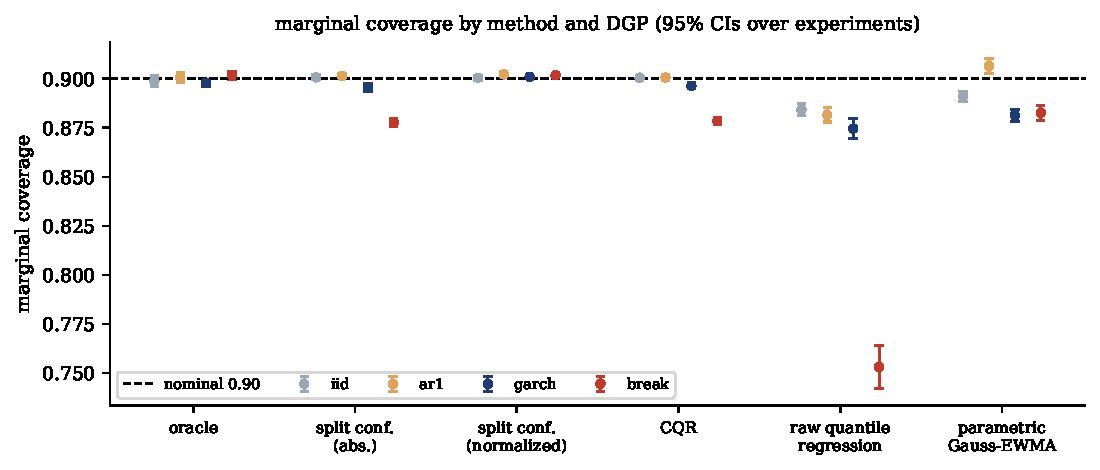
\includegraphics[width=\textwidth]{fig_marginal_coverage.pdf}
\caption{Marginal coverage by method and DGP with $95\%$ confidence intervals
over experiments (ACI omitted from the plot; it sits at $0.900$ everywhere,
Table~\ref{tab:marginal}). Stationary dependence (AR(1), GARCH) barely moves
the conformal methods; the break DGP dents the absolute-score and CQR
intervals and devastates the unconformalized quantile regression.}
\label{fig:marginal}
\end{figure}

\subsection{Conditional coverage is where it breaks---and normalization is the cheap fix}
\label{sec:conditional}

Marginal honesty can hide conditional dishonesty
\citep{lei2018distribution,christoffersen1998evaluating}. Stratifying GARCH
coverage by the \emph{true}-volatility tercile of each step
(Table~\ref{tab:conditional}, Figure~\ref{fig:conditional}) exposes the
headline failure: split conformal with the absolute score covers
$0.952/0.915/0.820$ across low/mid/high-volatility terciles---a spread of
$0.134$. The mechanism is structural, not statistical: the absolute score
produces an (essentially) constant-width interval, which is $1.39\times$ the
oracle width in the calm tercile and $0.89\times$ in the volatile one. The
interval is too wide exactly when wide intervals are cheap and too narrow
exactly when a position sizer needs the stated guarantee---under-covering by
$8$ points at nominal $90\%$.

Normalizing the score by the EWMA volatility closes most of the gap:
$0.893/0.905/0.905$, spread $0.040$. The paired per-experiment spread
reduction is $+0.094$ $[+0.076,+0.112]$, and the paired high-volatility
coverage gain is $+0.085$ $[+0.077,+0.093]$. CQR, often recommended as
\emph{the} heteroskedasticity fix, is only a partial one here:
$0.937/0.906/0.846$, spread $0.093$, a paired spread reduction of $+0.041$
$[+0.034,+0.049]$ and a high-volatility gain of $+0.027$
$[+0.021,+0.033]$---its gradient-boosted quantile learners react to the
volatility features too sluggishly, leaving high-volatility intervals at
$0.90\times$ the oracle width. Two honest footnotes to the headline. The
oracle itself shows a measured spread of $0.022$---the sampling floor of the
metric, against which the normalized score's $0.040$ should be read. And ACI
with an aggressive learning rate ($\gamma=0.05$, absolute score) also flattens
the terciles ($0.896/0.899/0.907$, spread $0.028$) by construction---it chases
its own misses---but does so at the price of $3.2\%$ unbounded intervals on
GARCH and a width that swings with the regime rather than tracking it.

\begin{table}[t]
\centering
\caption{Conditional coverage by true-volatility tercile on the GARCH DGP
($48$ experiments; nominal $0.90$). Spread is the per-experiment max--min
tercile coverage, averaged. Width ratios are relative to the oracle interval
within the tercile. The oracle row gives the sampling floor of both the
spread and the width metric.}
\label{tab:conditional}
\small
\begin{tabular}{lcccccc}
\toprule
& \multicolumn{3}{c}{Coverage by tercile} & & \multicolumn{2}{c}{Width / oracle}\\
\cmidrule(lr){2-4}\cmidrule(lr){6-7}
Method & low & mid & high & spread & low & high \\
\midrule
Oracle                              & 0.897 & 0.896 & 0.901 & 0.022 & 1.00 & 1.00 \\
Split conformal (absolute)          & 0.952 & 0.915 & 0.820 & 0.134 & 1.39 & 0.89 \\
Split conformal (normalized)        & 0.893 & 0.905 & 0.905 & 0.040 & 1.06 & 1.10 \\
CQR                                 & 0.937 & 0.906 & 0.846 & 0.093 & 1.24 & 0.90 \\
ACI, abs.\ score ($\gamma{=}0.05$)  & 0.896 & 0.899 & 0.907 & 0.028 & 1.08 & 1.11 \\
Raw quantile regression             & 0.928 & 0.887 & 0.808 & 0.120 & 1.17 & 0.81 \\
Parametric Gauss--EWMA              & 0.873 & 0.889 & 0.883 & 0.036 & 0.99 & 1.01 \\
\bottomrule
\end{tabular}
\end{table}

\begin{figure}[t]
\centering
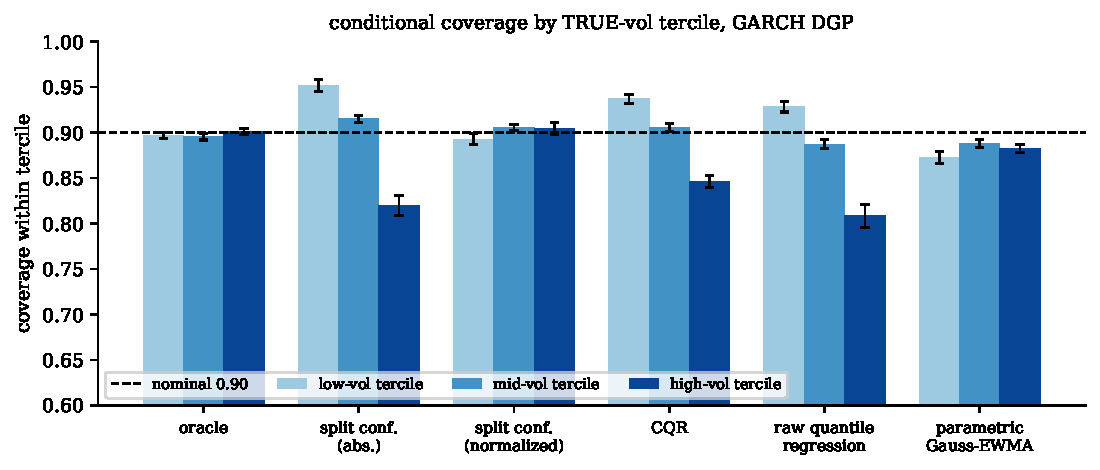
\includegraphics[width=\textwidth]{fig_conditional_coverage.pdf}
\caption{Conditional coverage by true-volatility tercile on the GARCH DGP
($95\%$ CIs over experiments). The absolute-score split conformal
over-covers calm regimes and under-covers volatile ones; the
volatility-normalized score is nearly flat at nominal; CQR closes less than
half the gap; the parametric Gauss--EWMA baseline is flat but sits uniformly
below nominal.}
\label{fig:conditional}
\end{figure}

\subsection{Breaks: the coverage hole, and what ACI buys}
\label{sec:breaks}

Table~\ref{tab:break} and Figure~\ref{fig:break} dissect the break DGP in
event time. Split conformal with the absolute score covers only $0.562$ over
the first $60$ post-break steps; its average hole depth (minimum rolling-$60$
coverage) is $0.543$ $[0.516,0.571]$. The hole is transient by mechanism: the
calibration window ($250$ steps) gradually fills with post-break scores, and
the rolling coverage is back above $0.87$ after a median of $191$ steps and
fully at nominal by steps $300$--$600$ ($0.901$). CQR behaves identically
($0.559$ first-$60$): conformalizing a quantile learner does not help when the
calibration distribution itself is stale. For calibration, note the oracle's
own hole depth is $0.801$ and its recovery time is $60$ (the metric's floor):
rolling-$60$ coverage dips that low on $90\%$-level Bernoulli noise alone.

The two repairs work, differently. \emph{Normalization} alone lifts the
first-$60$ coverage to $0.851$: $50$ of our $60$ realized breaks move volatility, the EWMA
proxy reacts within steps, and the normalized calibration scores stay nearly
exchangeable across the break. \emph{ACI} repairs by feedback, and its
learning rate buys speed monotonically: first-$60$ coverage
$0.700/0.777/0.839/0.875$ for $\gamma=0.005/0.01/0.02/0.05$ on the absolute
score, with recovery medians shrinking $93.5/77/66/61$ steps. The price is
width ($1.12$--$1.14\times$ oracle on the break DGP, versus $1.05\times$ for
plain split-absolute), occasional unbounded intervals ($3.0\%$ of steps at
$\gamma=0.05$), and post-hole \emph{over}-coverage while the loop pays back
its debt (up to $0.935$ at steps $150$--$300$ for $\gamma=0.005$)---the
long-run average is protected by oscillation, not by clairvoyance
\citep{gibbs2021adaptive,zaffran2022adaptive}. Stacking the fixes is best:
ACI on the \emph{normalized} score at $\gamma=0.01$ reaches $0.875$ in the
first $60$ steps and $0.924$ at $60$--$150$; at $\gamma=0.05$ it shows
essentially no hole at all ($0.900$ first-$60$; hole depth $0.847$, shallower
than the oracle's own $0.801$ noise floor) for $1.19\times$ oracle width and
$0.7\%$ unbounded steps. The unconformalized quantile regression, for contrast, never really
recovers: $0.459$ in the first $60$ steps, still $0.671$ at $300$--$600$, and
only $86.7\%$ of its paths ever regain the $0.87$ threshold.

\begin{table}[t]
\centering
\caption{Post-break behavior on the break DGP ($60$ experiments). Event-time
coverage windows are steps since the break; hole depth is the minimum
rolling-$60$ coverage after the break; recovery is the median first step at
which rolling-$60$ coverage returns above $0.87$ ($60$ is the metric's floor),
computed among runs that recover, with the recovered fraction reported
alongside; width is the mean ratio to the oracle over the bounded steps of
the test segment (the unbounded fraction is reported separately). The oracle
row calibrates the noise floor of the event-time metrics.}
\label{tab:break}
\vspace{4pt}
\small
\begin{tabular}{lcccccc}
\toprule
& \multicolumn{3}{c}{Coverage in window} & & & \\
\cmidrule(lr){2-4}
Method & 0--60 & 60--150 & 300--600 & hole & recovery & width \\
\midrule
Oracle                          & 0.896 & 0.910 & 0.896 & 0.801 & 60    & 1.00 \\
Split conformal (absolute)      & 0.562 & 0.764 & 0.901 & 0.543 & 191   & 1.05 \\
Split conformal (normalized)    & 0.851 & 0.922 & 0.903 & 0.816 & 64.5  & 1.14 \\
CQR                             & 0.559 & 0.771 & 0.902 & 0.540 & 190.5 & 1.03 \\
ACI abs., $\gamma{=}0.005$      & 0.700 & 0.909 & 0.916 & 0.694 & 93.5  & 1.12 \\
ACI abs., $\gamma{=}0.01$       & 0.777 & 0.923 & 0.906 & 0.771 & 77    & 1.12 \\
ACI abs., $\gamma{=}0.02$       & 0.839 & 0.914 & 0.902 & 0.819 & 66    & 1.12 \\
ACI abs., $\gamma{=}0.05$       & 0.875 & 0.907 & 0.901 & 0.843 & 61    & 1.14 \\
ACI norm., $\gamma{=}0.01$      & 0.875 & 0.924 & 0.898 & 0.820 & 60    & 1.14 \\
Raw quantile regression         & 0.459 & 0.445 & 0.671 & 0.326 & 601.5 & 0.81 \\
Parametric Gauss--EWMA          & 0.664 & 0.823 & 0.903 & 0.647 & 149.5 & 1.09 \\
\bottomrule
\end{tabular}
\end{table}

\begin{figure}[t]
\centering
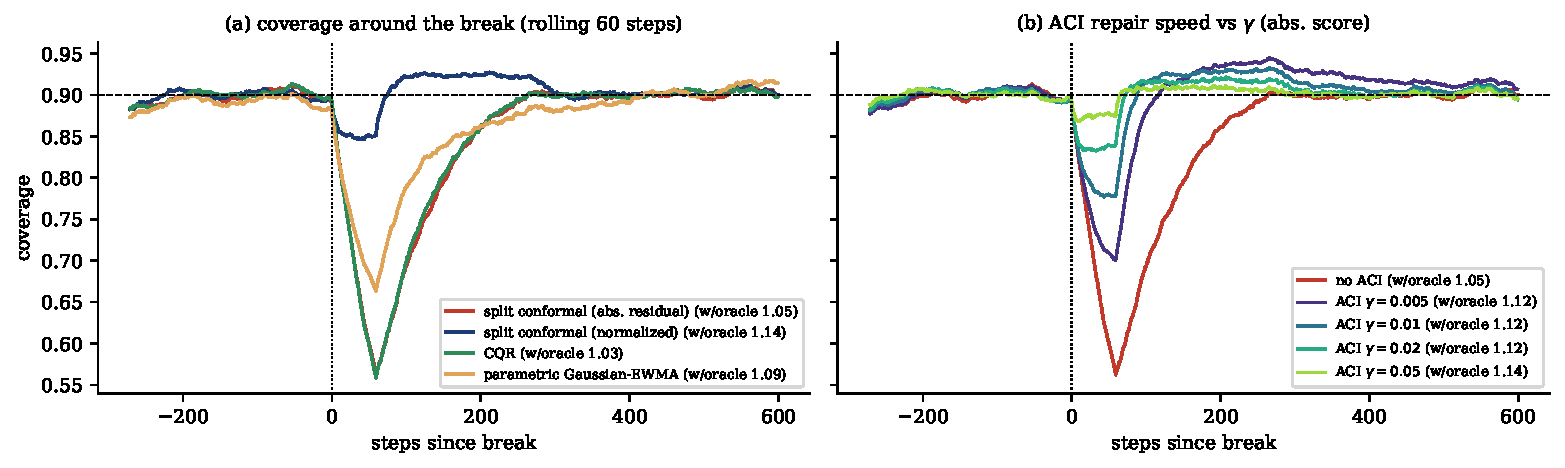
\includegraphics[width=\textwidth]{fig_break_aci.pdf}
\caption{Event-time coverage around the break (rolling $60$ steps, averaged
over the $60$ break experiments; legend gives each method's mean
width-to-oracle ratio). (a) Split-absolute and CQR dig the same deep hole and
climb out only as the calibration window turns over; volatility normalization
almost removes the hole; the parametric Gauss--EWMA falls in between. (b) ACI
on the absolute score: repair speed is monotone in $\gamma$, and the
small-$\gamma$ variants overshoot above nominal after the hole while the
long-run average is restored.}
\label{fig:break}
\end{figure}

\subsection{Width at matched coverage: what honesty costs, and what narrowness hides}
\label{sec:width}

Coverage comparisons are only meaningful at matched coverage, so we compare
widths among methods whose marginal coverage falls in the band
$[0.885,0.915]$, separately by DGP and innovation family. On GARCH---the
economically central case---the conformal premium over the oracle width is:
split-absolute $1.15\times$ (Gaussian innovations) and $1.13\times$
(Student-$t$); normalized $1.09\times$/$1.08\times$; CQR
$1.08\times$/$1.06\times$. The parametric Gauss--EWMA baseline is the
narrowest interval in the comparison, $0.99\times$/$1.03\times$---but its
coverage there is $0.878$/$0.888$, below the band's lower edge in the Gaussian
cell and barely inside it under Student-$t$. Its narrowness is not
efficiency; it is under-coverage wearing efficiency's clothes. The
unconformalized quantile regression tells the same story at $0.99\times$ width
and $0.871$--$0.880$ coverage. Across all eight DGP$\times$innovation cells,
no method inside the coverage band is narrower than the oracle.

Two practical readings. First, on heteroskedastic data the normalized score
is not just the conditional-coverage fix (Section~\ref{sec:conditional})---it
is also \emph{cheaper} than the absolute score at matched marginal coverage
($1.08$--$1.09\times$ vs $1.13$--$1.15\times$), because matching the oracle's
shape lets it match the oracle's average width more closely. There is no
width-vs-honesty trade-off in choosing it. Second, the honest premium for
distribution-free finite-sample coverage on GARCH is roughly $6$--$9\%$ of
interval width (normalized or CQR) over an oracle no real forecaster
possesses---a modest insurance premium against the parametric alternative's
silent $1$--$2$-point coverage shortfall.

\subsection{Fat tails are not why the Gaussian baseline fails at 90\%}
\label{sec:tails}

A folklore argument says Gaussian intervals under-cover financial returns
because returns are fat-tailed. At the $90\%$ level this is backwards. The
central $90\%$ interval is set by the $0.95$ quantile, and for
\emph{standardized} (unit-variance) Student-$t$ innovations that quantile is
\emph{smaller} than the Gaussian $1.645$: $1.507/1.587/1.621$ for
$\nu=4/6/10$. Fat tails move mass from the shoulders to both the tails and
the center; at central coverage levels the center wins, and a correctly-scaled
Gaussian interval \emph{over}-covers. The ordering only flips deep in the
tails (at the $0.995$ quantile: $3.256$ vs.\ $2.576$ for $\nu=4$), which is
where the folklore belongs---VaR at $99\%$+, not $90\%$ intervals.

Our measurements bear this out: the parametric baseline covers slightly
\emph{more} under Student-$t$ innovations than under Gaussian ones ($0.894$
vs.\ $0.888$ on iid; $0.888$ vs.\ $0.878$ on GARCH), the opposite of the
folklore's prediction. Its under-coverage is instead driven by volatility
dynamics---estimation noise in the EWMA filter on iid data, filter lag under
GARCH, and stale variance after breaks ($0.664$ in the first $60$ post-break
steps)---failure modes that conformal calibration absorbs and a plug-in
$z$-score does not. Practitioners patching a Gaussian interval for ``fat
tails'' at the $90\%$ level are treating the wrong disease.

\section{Discussion}
\label{sec:discussion}

\paragraph{A practical recipe.} The results compose into a simple default for
return intervals at central coverage levels. (1) Always conformalize: the raw
quantile-regression band gives up $1.6$--$2.5$ coverage points on stationary
DGPs and $15$ points after breaks, while calibration costs one data split.
(2) Normalize the score by a volatility proxy---even a fixed-decay EWMA. It
closes the conditional-coverage spread from $0.134$ to $0.040$, repairs most
of the volatility-break hole ($0.851$ vs.\ $0.562$ first-$60$ coverage), keeps
marginal coverage at nominal on every DGP we tested, and is \emph{narrower}
than the absolute score at matched coverage on heteroskedastic data. It is
the rare free lunch in this menu. (3) If regime breaks are a first-order
concern, add ACI on top of the normalized score, choosing $\gamma$ by the
hole-vs-oscillation trade-off of Table~\ref{tab:break}; $\gamma\approx0.01$
already cuts the hole substantially at negligible marginal-width cost, and
$\gamma=0.05$ eliminates it at ${\sim}1.19\times$ oracle width with a small
fraction of unbounded steps that a deployment must handle (cap the width or
abstain). CQR is a reasonable method, but on these DGPs it neither matches
the normalized score conditionally nor survives breaks better than the
absolute score, so it is not the first tool we would reach for.

\paragraph{What conformal buys against a parametric volatility model.} The
Gauss--EWMA baseline embodies the econometric default: model the variance,
plug in a quantile. When its assumptions are close to true it is the
narrowest interval on offer---and it still under-covered in six of our eight
DGP$\times$innovation cells, because estimation noise, filter lag, and breaks
all push the same direction and nothing in the plug-in construction pushes
back. Conformal calibration is exactly that counter-pressure: it converts
\emph{whatever} interval shape one believes in (including the parametric one)
into a coverage-honest version of itself for a $6$--$9\%$ width premium. The
right mental model is not ``conformal vs.\ GARCH'' but ``calibrated vs.\
uncalibrated'': normalize by the best volatility estimate available, then let
the calibration set vote on the quantile. When the volatility model is good,
the premium is small; when it is wrong, the calibration step is what keeps the
stated $90\%$ meaning $90\%$---marginally always, conditionally if the
normalizer tracks the regime, and after breaks if ACI is listening.

\section{Limitations}
\label{sec:limitations}

Everything here is simulation, by design: exact conditional truth is the point
of the paper and is unobtainable on market data. The cost is a list of
simplifications, all visible in the released code. The DGP menu---iid, AR(1)
mean, GARCH(1,1), single abrupt break, with Gaussian or standardized
Student-$t$ innovations---omits leverage effects, jumps, skewed innovations,
long memory, and recurring or gradual regime shifts. We study one asset and
one horizon (one-step-ahead); cross-sectional and multi-horizon questions are
out of scope. The learners are gradient-boosting machines with fixed,
untuned hyperparameters ($100$ trees, depth $2$, learning rate $0.08$); a
stronger or better-tuned quantile learner would likely improve CQR
specifically, and our ranking of CQR versus the normalized score should be
read with that asymmetry in mind. The online protocol fixes one cadence
(refit every $250$ steps, train $600$, calibrate $250$); the post-break
recovery time scales with the calibration window by mechanism, so these
constants shape the transient results. The parametric baseline is a
QML-fitted EWMA filter, not a full GARCH(1,1) maximum-likelihood fit; on the
GARCH DGP a correctly-specified MLE baseline would be stronger, though it
would not change the structural point that plug-in intervals lack a
calibration feedback. The nominal level is $0.90$ throughout; at deeper tail
levels (e.g.\ $99\%$+) the fat-tail ordering of Section~\ref{sec:tails}
reverses and several conclusions about the Gaussian baseline would
quantitatively change. Finally, confidence intervals are normal
approximations over independent experiments, appropriate for the $36$--$60$
replications per DGP but not a substitute for exact inference.

\section{Conclusion}
\label{sec:conclusion}

We measured what conformal prediction actually delivers on financial-return
DGPs where the truth is known. Marginal coverage survives stationary
dependence almost exactly---the exchangeability gap is $-0.005$ under GARCH
and invisible under AR(1)---so the common warning that serial dependence
voids conformal guarantees is, marginally and at this scale, overstated.
What breaks is everything a risk manager actually cares about beyond the
average: the absolute-score interval under-covers high-volatility regimes by
$8$ points while over-covering calm ones by $5$, and abrupt breaks open a
coverage hole that reaches $0.562$ over the first $60$ steps and heals only
as fast as the calibration window. Both failures have cheap, composable
fixes: an EWMA-normalized score (spread $0.134\to0.040$; hole
$0.562\to0.851$; marginal coverage intact everywhere; narrower at matched
coverage), and ACI for the residual break risk (hole repair monotone in
$\gamma$ at a $1.12$--$1.14\times$ width cost, long-run coverage $0.900$ by
theorem and by measurement). The parametric Gaussian--EWMA alternative is
narrower than every honest method---because it under-covers; its narrowness
is bought with coverage, and its failures at the $90\%$ level stem from
volatility dynamics, not the fat tails folklore blames. Conformal prediction
for returns is neither a guarantee that transfers unscathed nor a method
broken by dependence: it is a calibration layer whose marginal promise is
cheap to keep, whose conditional promise must be \emph{earned} with a
volatility-aware score, and whose post-break promise needs a feedback loop.
Used that way, it turns a $6$--$9\%$ width premium into intervals whose
stated level survives the regimes where parametric confidence quietly fails.

\paragraph{Reproducibility.} All experiments are deterministic given the
released seed ($20260610$). The script \texttt{scripts/run\_all.py}
regenerates every record, summary, and number in this paper
(\texttt{results/results.json}, \texttt{records.csv}; about six minutes on one
core), \texttt{python -m conformal\_experiments.figures} regenerates all four
figures, \texttt{scripts/check\_paper\_numbers.py} asserts that every number
quoted in this paper matches the generated results, and a $17$-test suite
checks the DGP ground truths and the conformal theorems (including the ACI
update direction). The DGPs, methods, protocol, and analysis are released as
an open-source package at the repository above.

\small
\bibliographystyle{plainnat}
\bibliography{refs}

\end{document}
